\documentclass[xcolor=x11names,compress,professionalfonts]{beamer}

%% General packages %%%%%%%%%%%%%%%%%%%%%%%%%%%%%%%%%%
\usepackage[utf8]{inputenc}
\usepackage{graphicx}
\usepackage{tikz}
\tikzset{% change default arrow tips
    >=latex
}
\usepackage{ifthen}

\usepackage{amsmath}
\usepackage{nicefrac}

\usepackage{color}

%%%%%%%%%%%%%%%%%%%%%%%%%%%%%%%%%%%%%%%%%%%%%%%%%%%%%%


%% Beamer Layout %%%%%%%%%%%%%%%%%%%%%%%%%%%%%%%%%%
\useoutertheme[subsection=false,shadow]{miniframes}
\useinnertheme{rectangles}

\setbeamertemplate{navigation symbols}{}%remove navigation symbols

\newcommand{\btVFill}{\vskip0pt plus 1filll}%place an element at the bottom of the page

\usepackage{libertine}
\usepackage[T1]{fontenc}

\setbeamerfont{title like}{shape=\scshape}
\setbeamerfont{frametitle}{shape=\scshape}

\setbeamercolor*{lower separation line head}{bg=DeepSkyBlue4} 
\setbeamercolor*{normal text}{fg=black,bg=white} 
\setbeamercolor*{alerted text}{fg=red} 
\setbeamercolor*{example text}{fg=black} 
\setbeamercolor*{structure}{fg=black} 
 
\setbeamercolor*{palette tertiary}{fg=black,bg=black!10} 
\setbeamercolor*{palette quaternary}{fg=black,bg=black!10} 

\renewcommand{\(}{\begin{columns}}
\renewcommand{\)}{\end{columns}}
\newcommand{\<}[1]{\begin{column}{#1}}
\renewcommand{\>}{\end{column}}

\definecolor{BostonBlue}{HTML}{00688B}
\definecolor{Complementary}{HTML}{8B2300}

\renewcommand{\ss}[1]{\scriptsize{\text{#1}}}
%%%%%%%%%%%%%%%%%%%%%%%%%%%%%%%%%%%%%%%%%%%%%%%%%%

\usepackage{braket}
% compile child documents using this preamble
\usepackage{subfiles}

%%%My Math

\newcommand{\pd}[2]{\frac{\displaystyle \partial #1}{\displaystyle\partial #2}} % for partial derivatives
\renewcommand{\d}[1]{\mathrm{d}#1}

\begin{document}

\begin{frame}
\title{Fractal states on quasicrystals}

\author{ Nicolas Macé}

\institute % (optional)
{
  Laboratoire de Physique des Solides
}

\date{January 20, 2016}

\titlepage

\btVFill
\centering
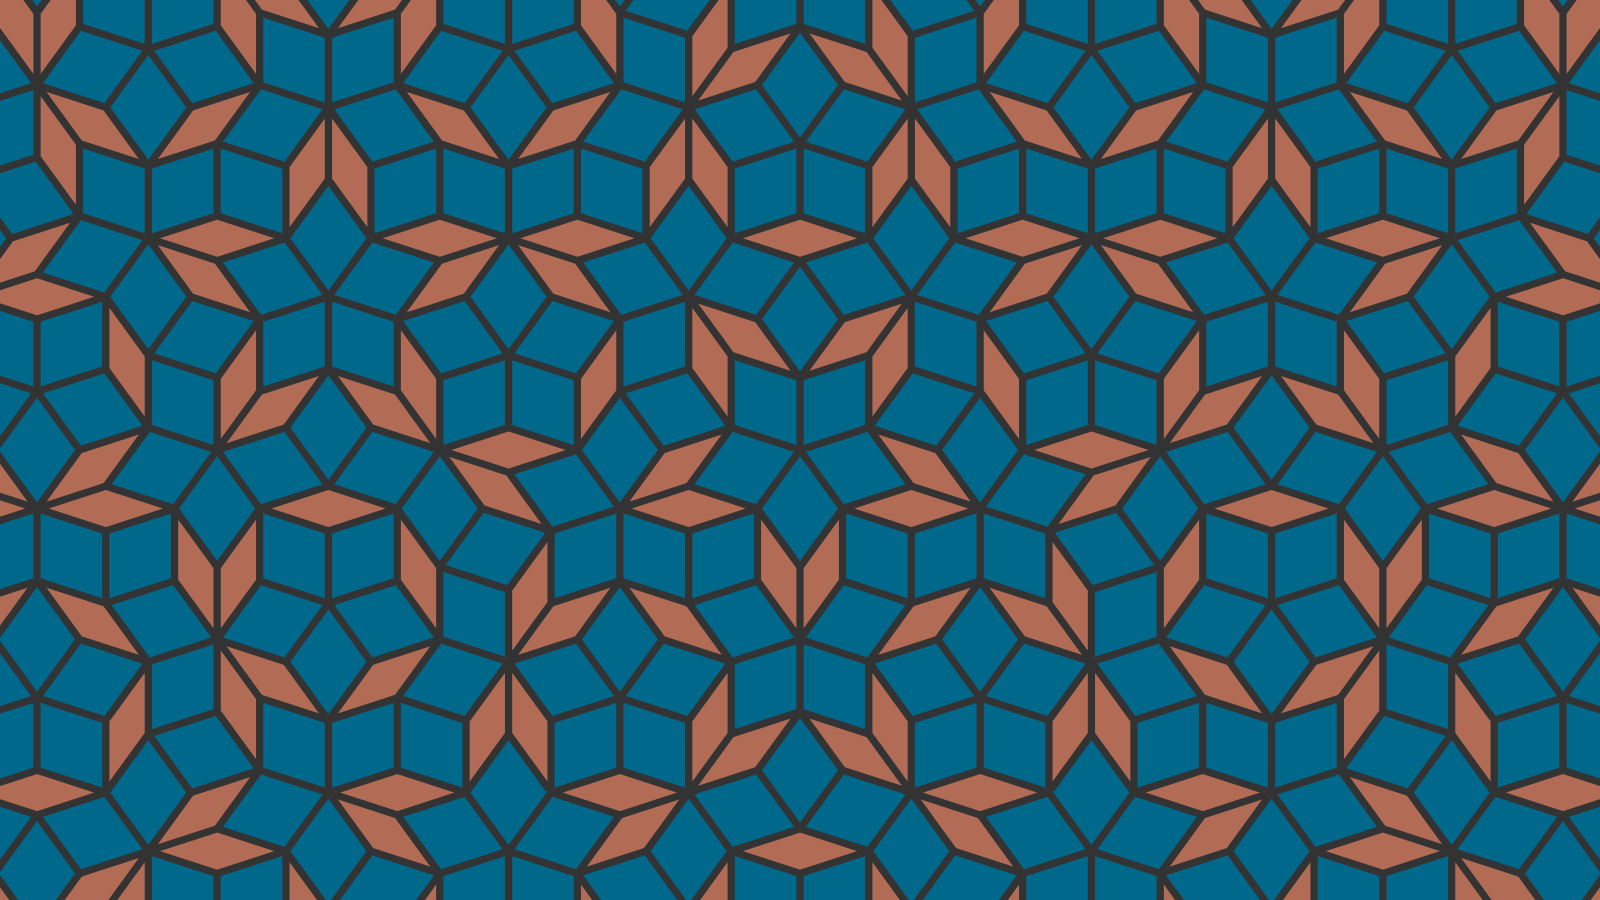
\includegraphics[scale=0.12]{img/cover.png}

\end{frame}

\begin{frame}
\frametitle{Outline}
\tableofcontents[hideallsubsections]
\end{frame}

\section{Quasicrystals and their physical properties}
%Each section needs a subsection for the small points on top to show up
\subsection{Dummy}
\begin{frame}{Quasicrystal?}
A crystalline structure based on a quasiperiodic tiling. 

A qp tiling is required to:
\begin{itemize}
	\item fill space (tiling)
	\item be \textbf{aperiodic} (a translate of the tiling does not superpose with the tiling itself)
	\item have \textbf{some kind of long range order} (diffraction reveals sharp peaks)
\end{itemize}

\(
	\<{6cm}
		\centering
		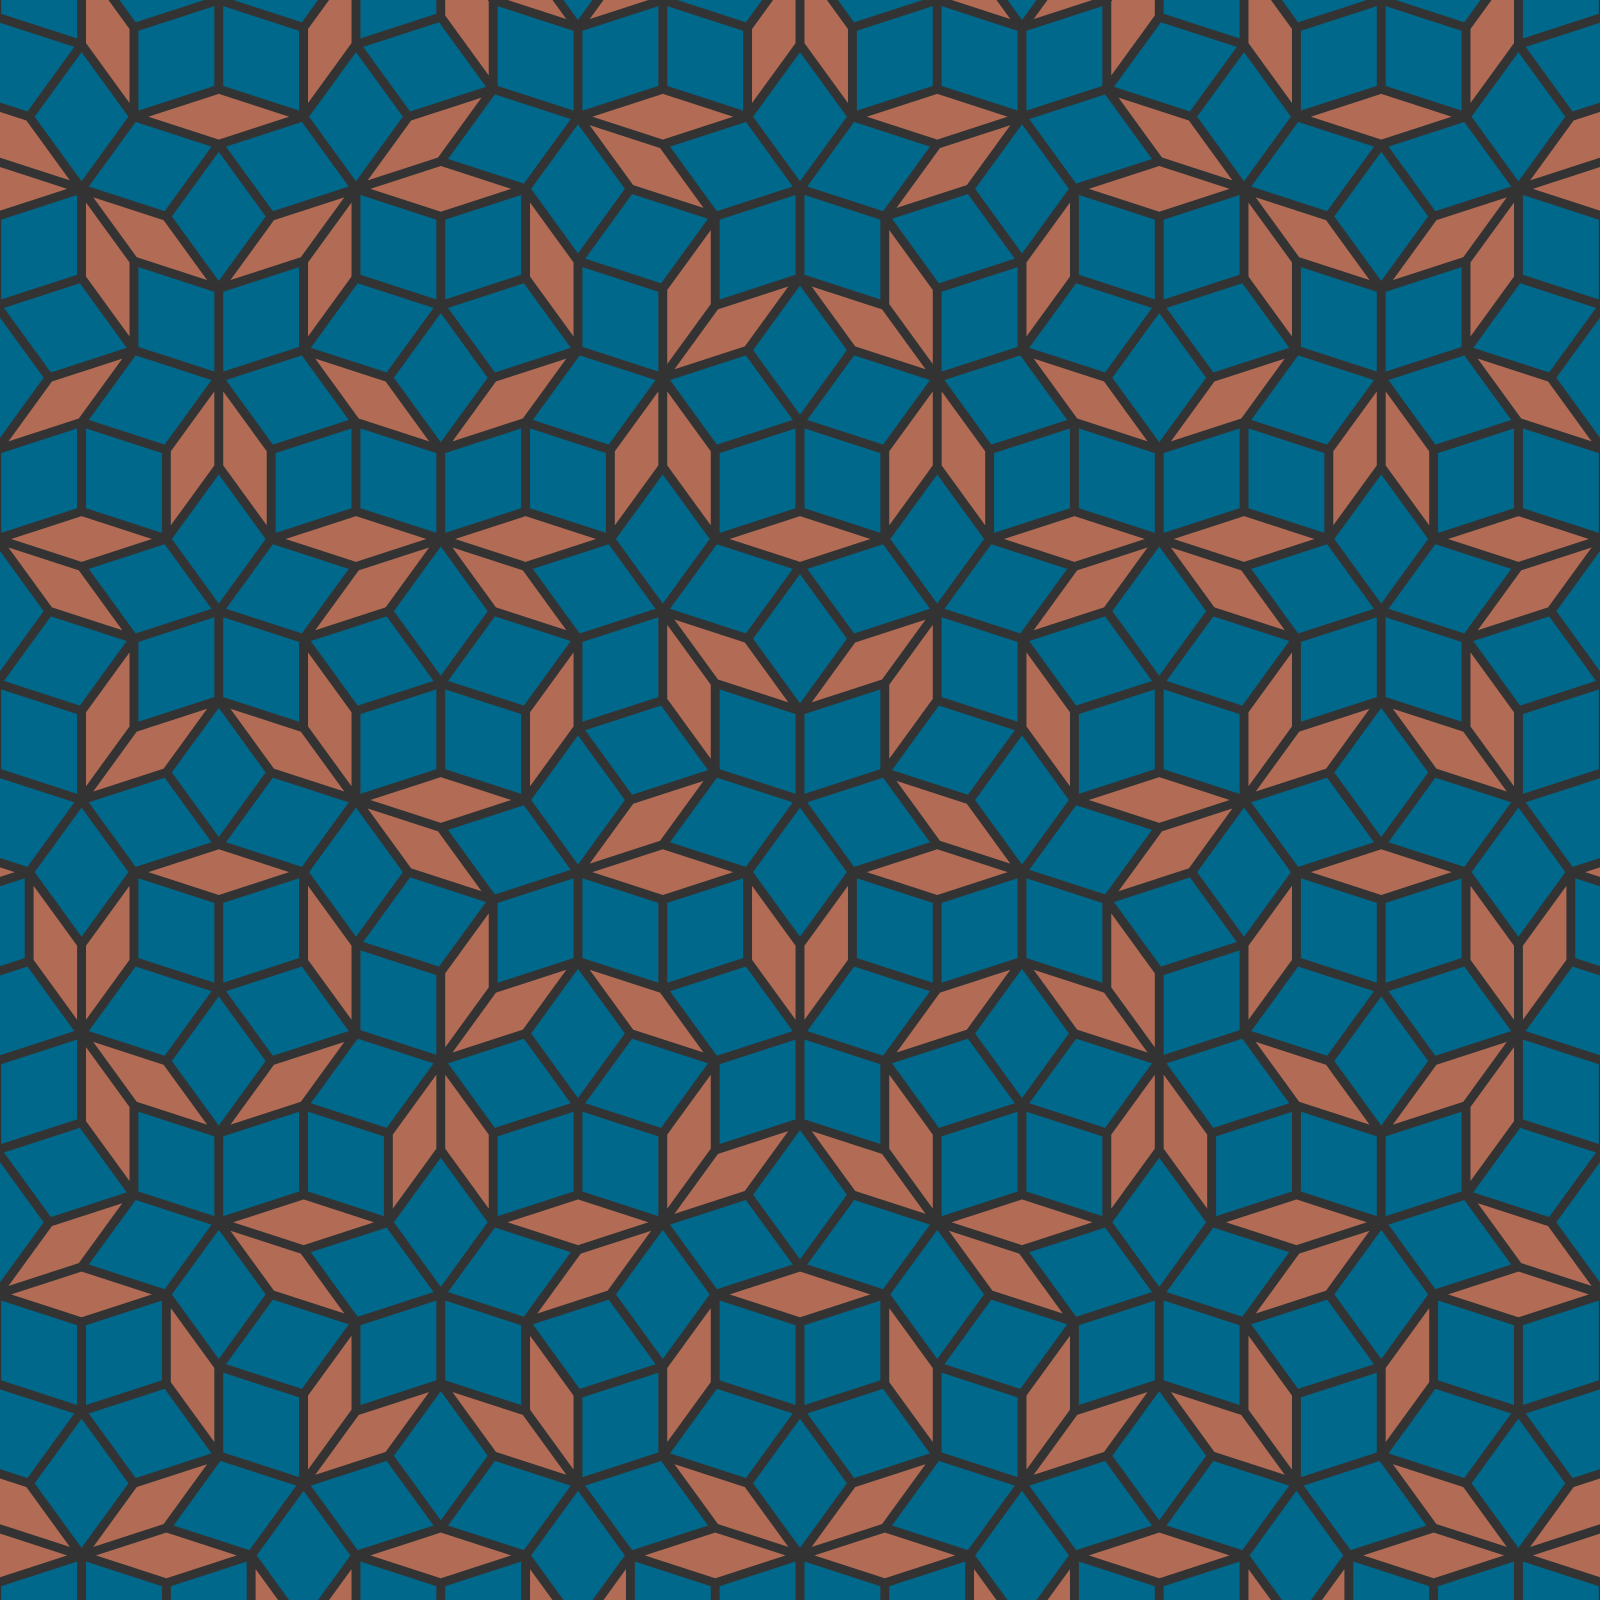
\includegraphics[scale=0.06]{img/penrose.png}
		
		\ss{A patch of the Penrose tiling,} \ss{which has an order 5 rotational symmetry}
	\>
	\<{6cm}
		\centering
		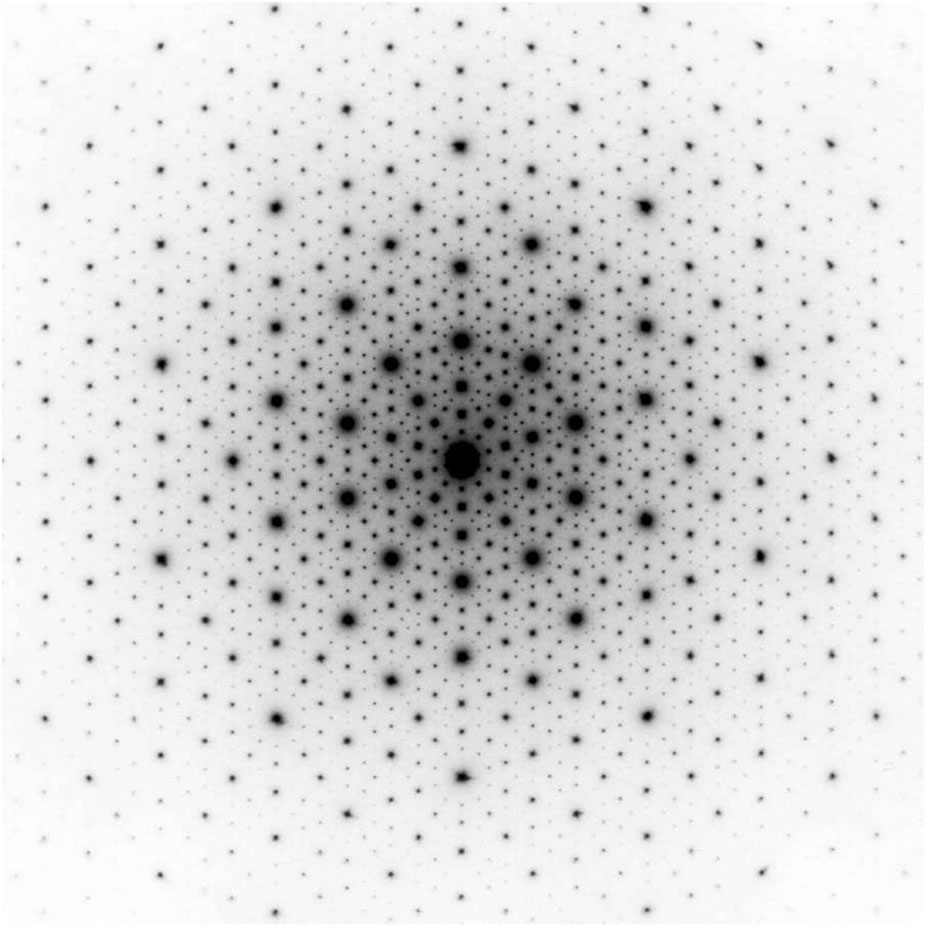
\includegraphics[scale=0.1]{img/diffraction_tenfold.png}
		
		\ss{Experimental diffraction pattern of AlPdMn} \ss{(Conradin Beeli group)}
	\>
\)
\end{frame}

\begin{frame}{A recipe for bulding quasiperiodic lattices}
Take a \textbf{periodic lattice}, cut a slice in it, project the selected points on a ``physical'' hyperplane.
\begin{figure}[htp]
\centering
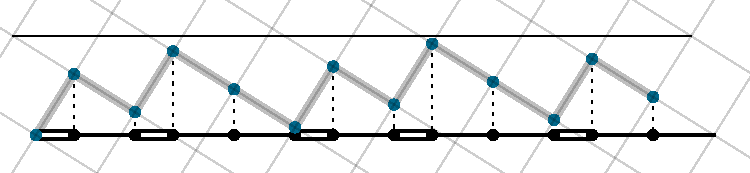
\includegraphics[scale=.6]{img/cut_and_project_Fibonacci.pdf}

\ss{A one dimensional quasicrystal, built from a 2D square lattice.}

\(
	\<{6cm}
		\centering
		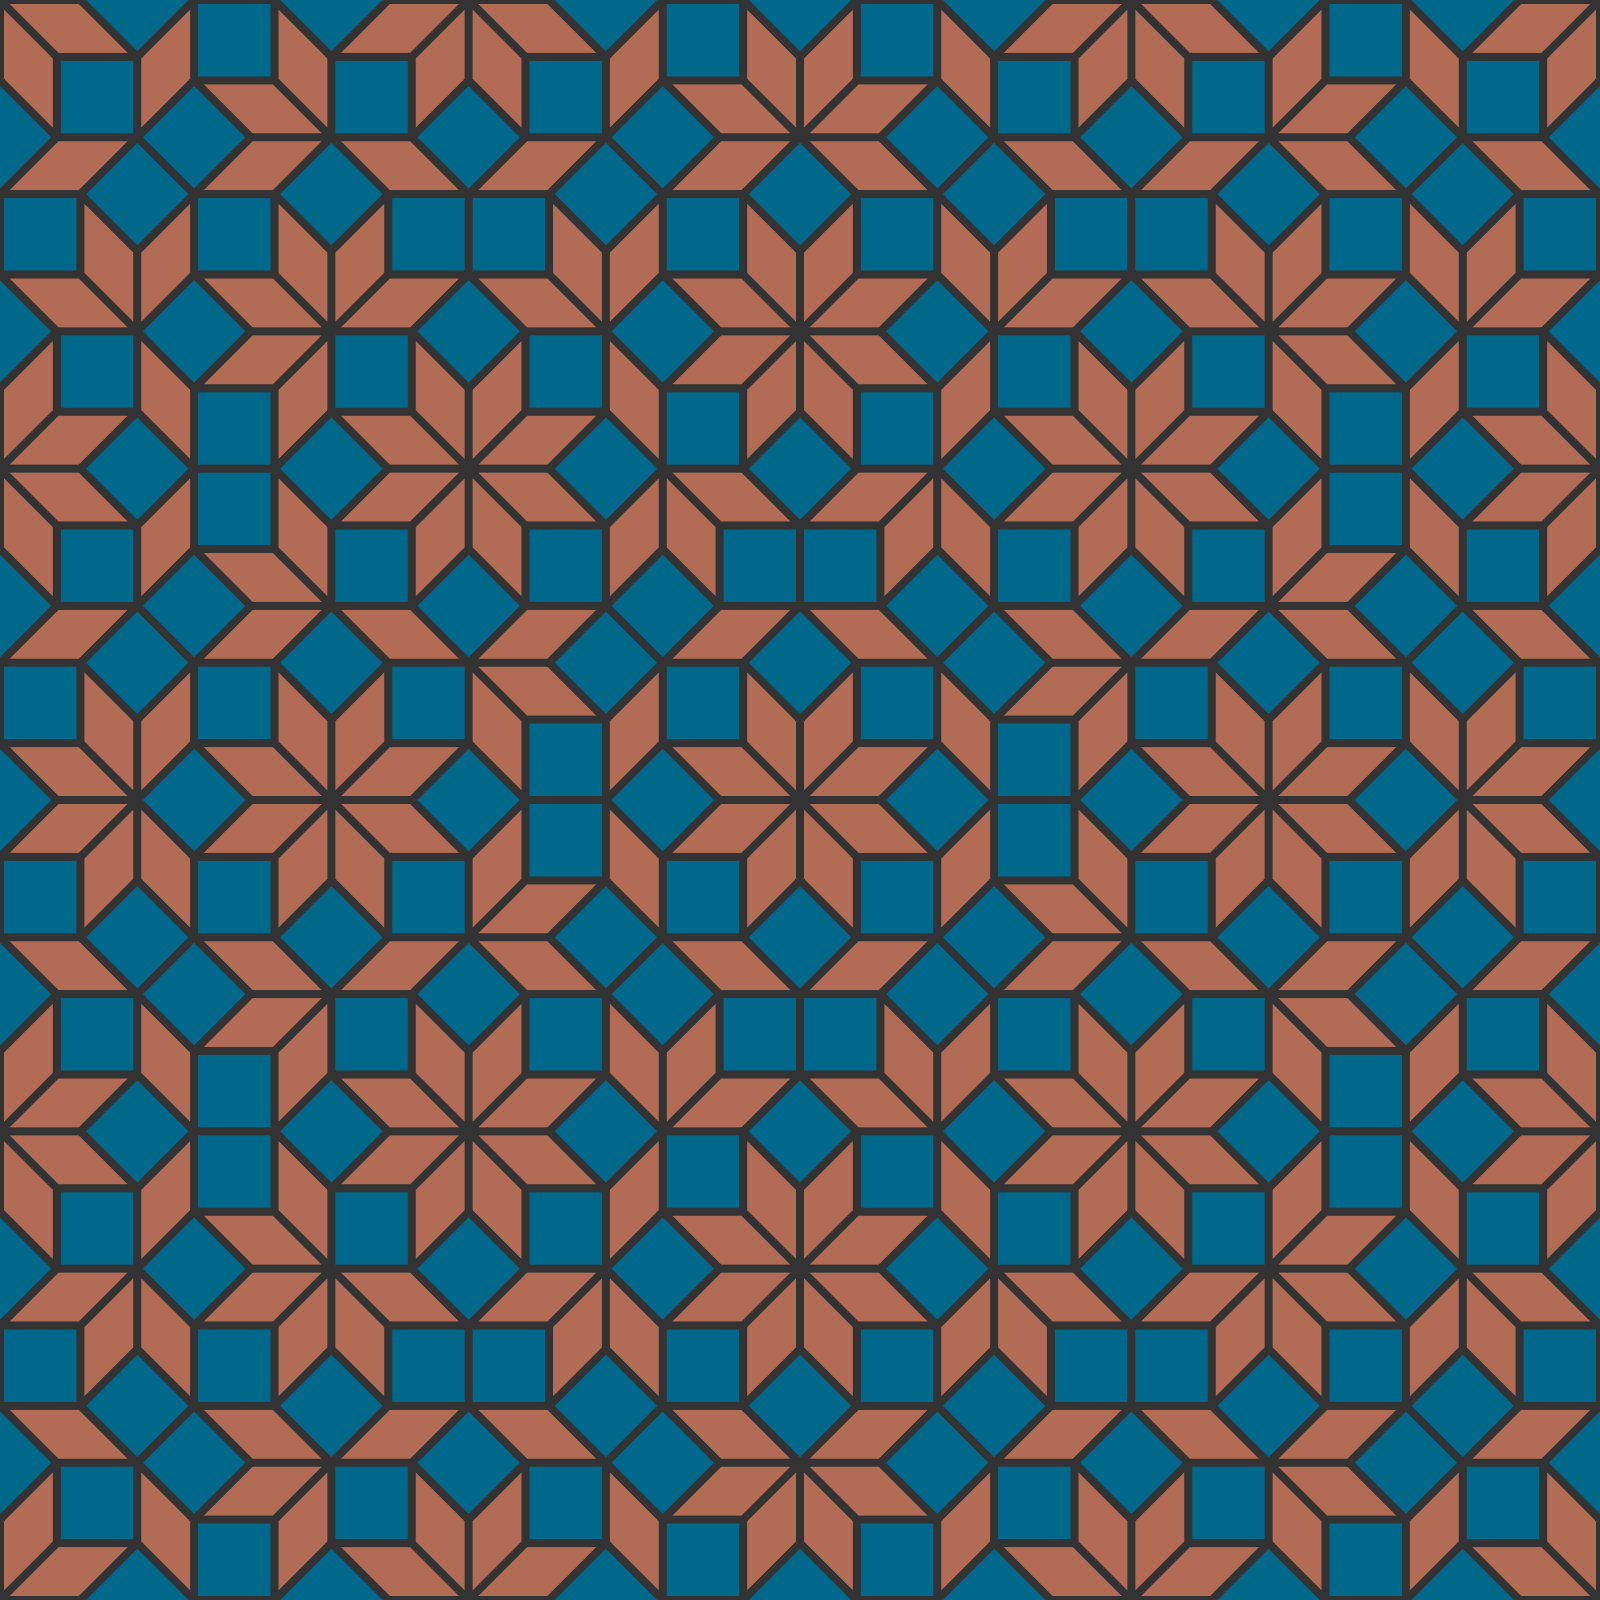
\includegraphics[scale=0.07]{img/ammann-beenker.png}
		
		\ss{The octagonal tiling,} \ss{built from a 4D square lattice.}
	\>
	\<{6cm}
		\centering
		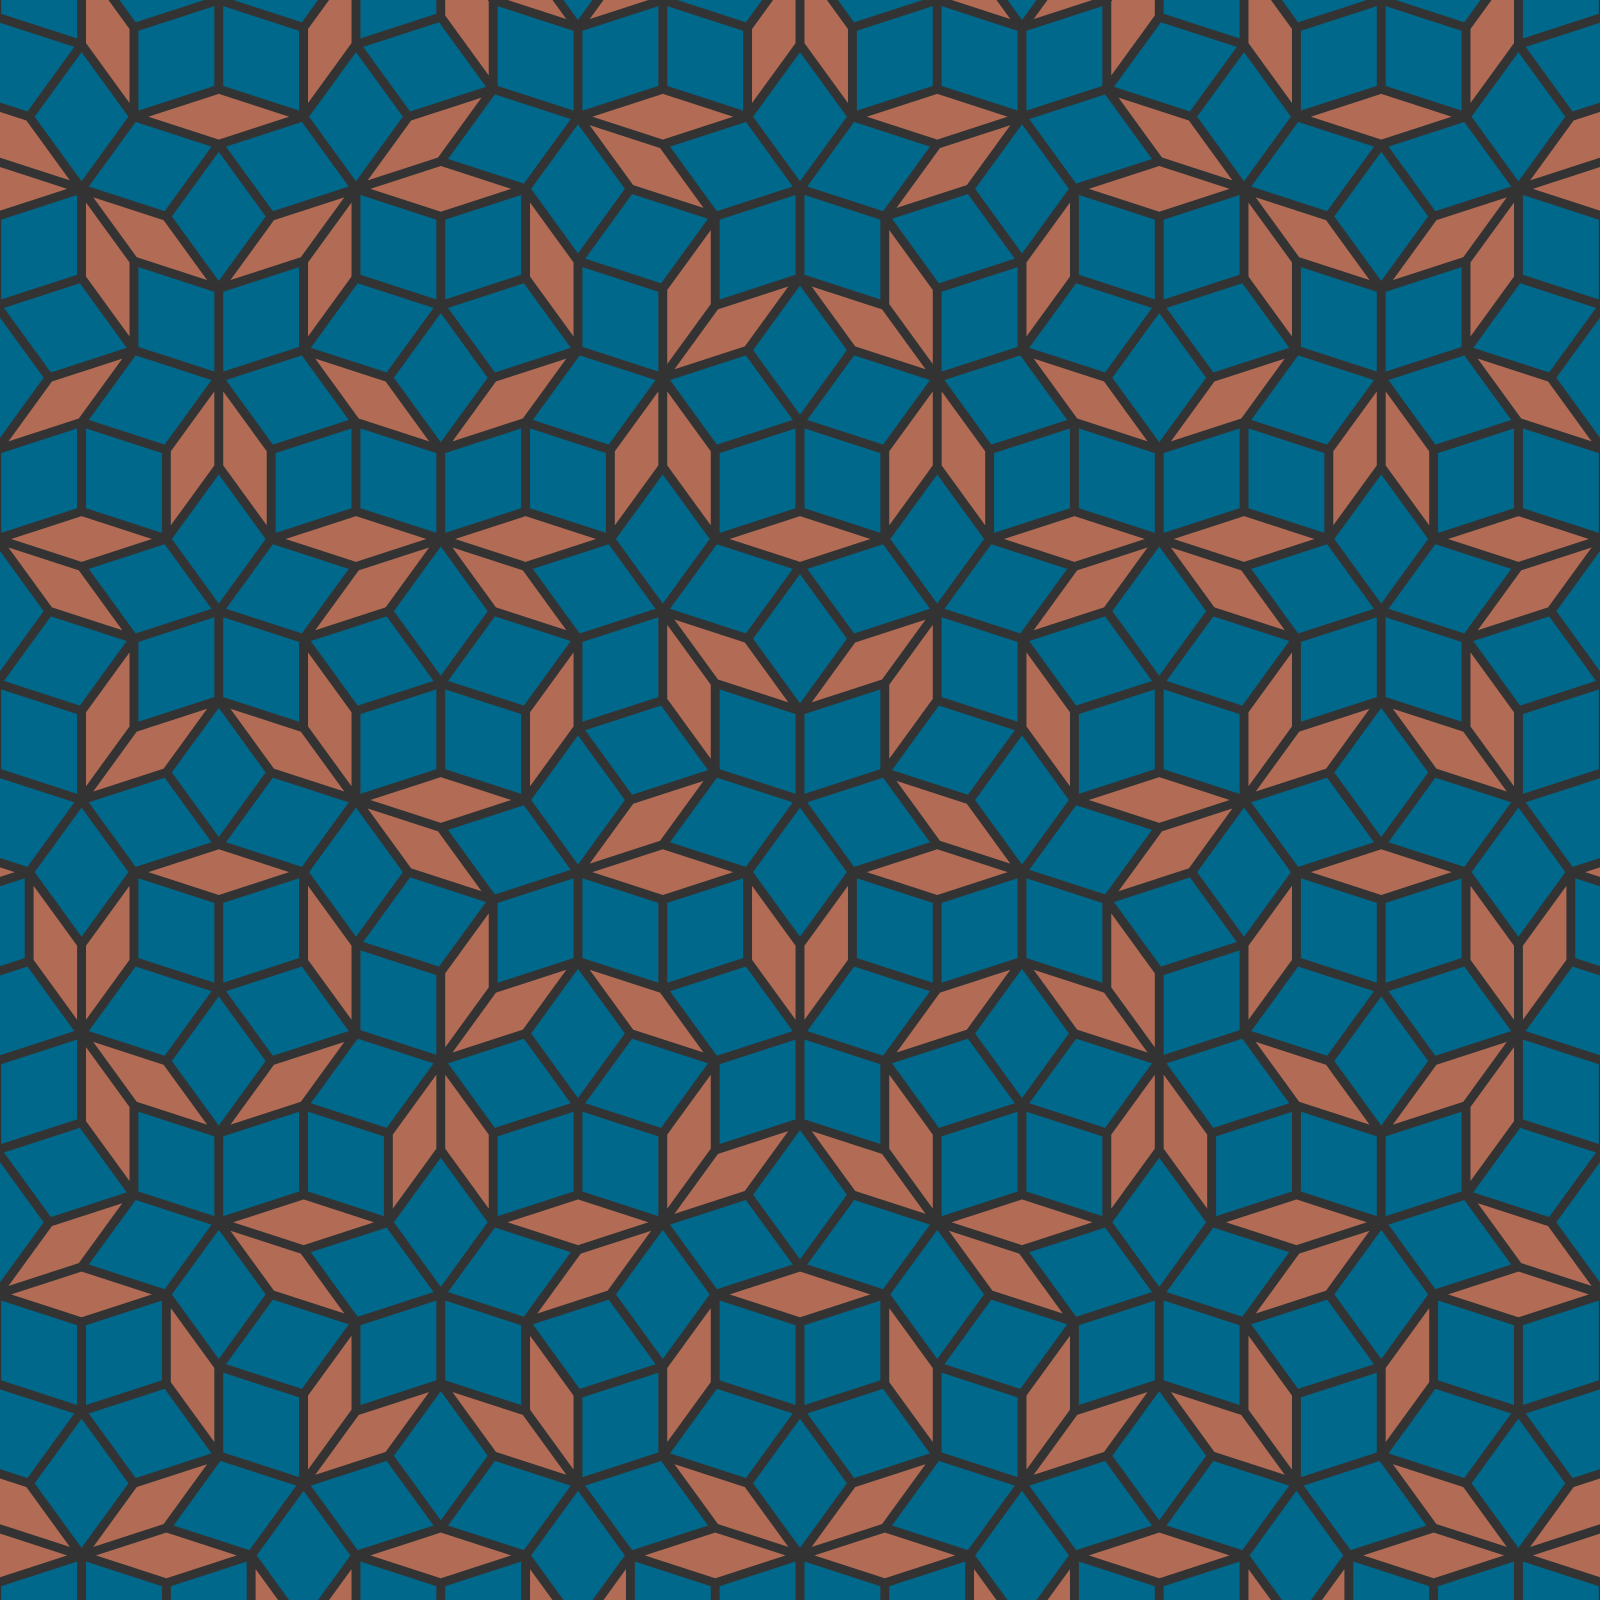
\includegraphics[scale=0.07]{img/penrose.png}
		
		\ss{The Penrose tiling, built} \ss{from a 5D square lattice.}
	\>
\)
\end{figure}
\end{frame}

\begin{frame}{Real life examples}
\(
	\<{6cm}
		\centering
		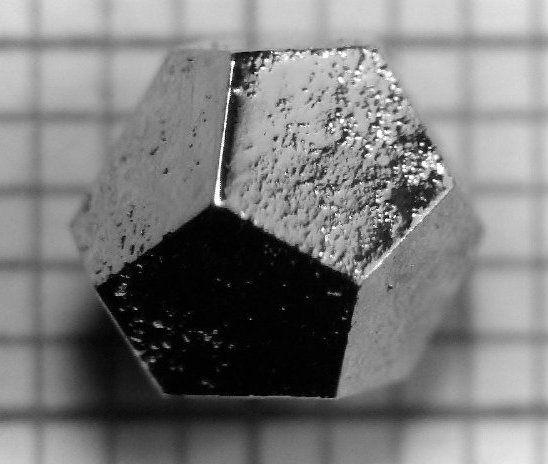
\includegraphics[scale=0.28]{img/homgzn.png}
		
		\ss{HoMgZn alloy in its icosahedral phase} \ss{(see \url{doi:10.1038/nmat1244})}
	\>
	\<{6cm}
		\centering
		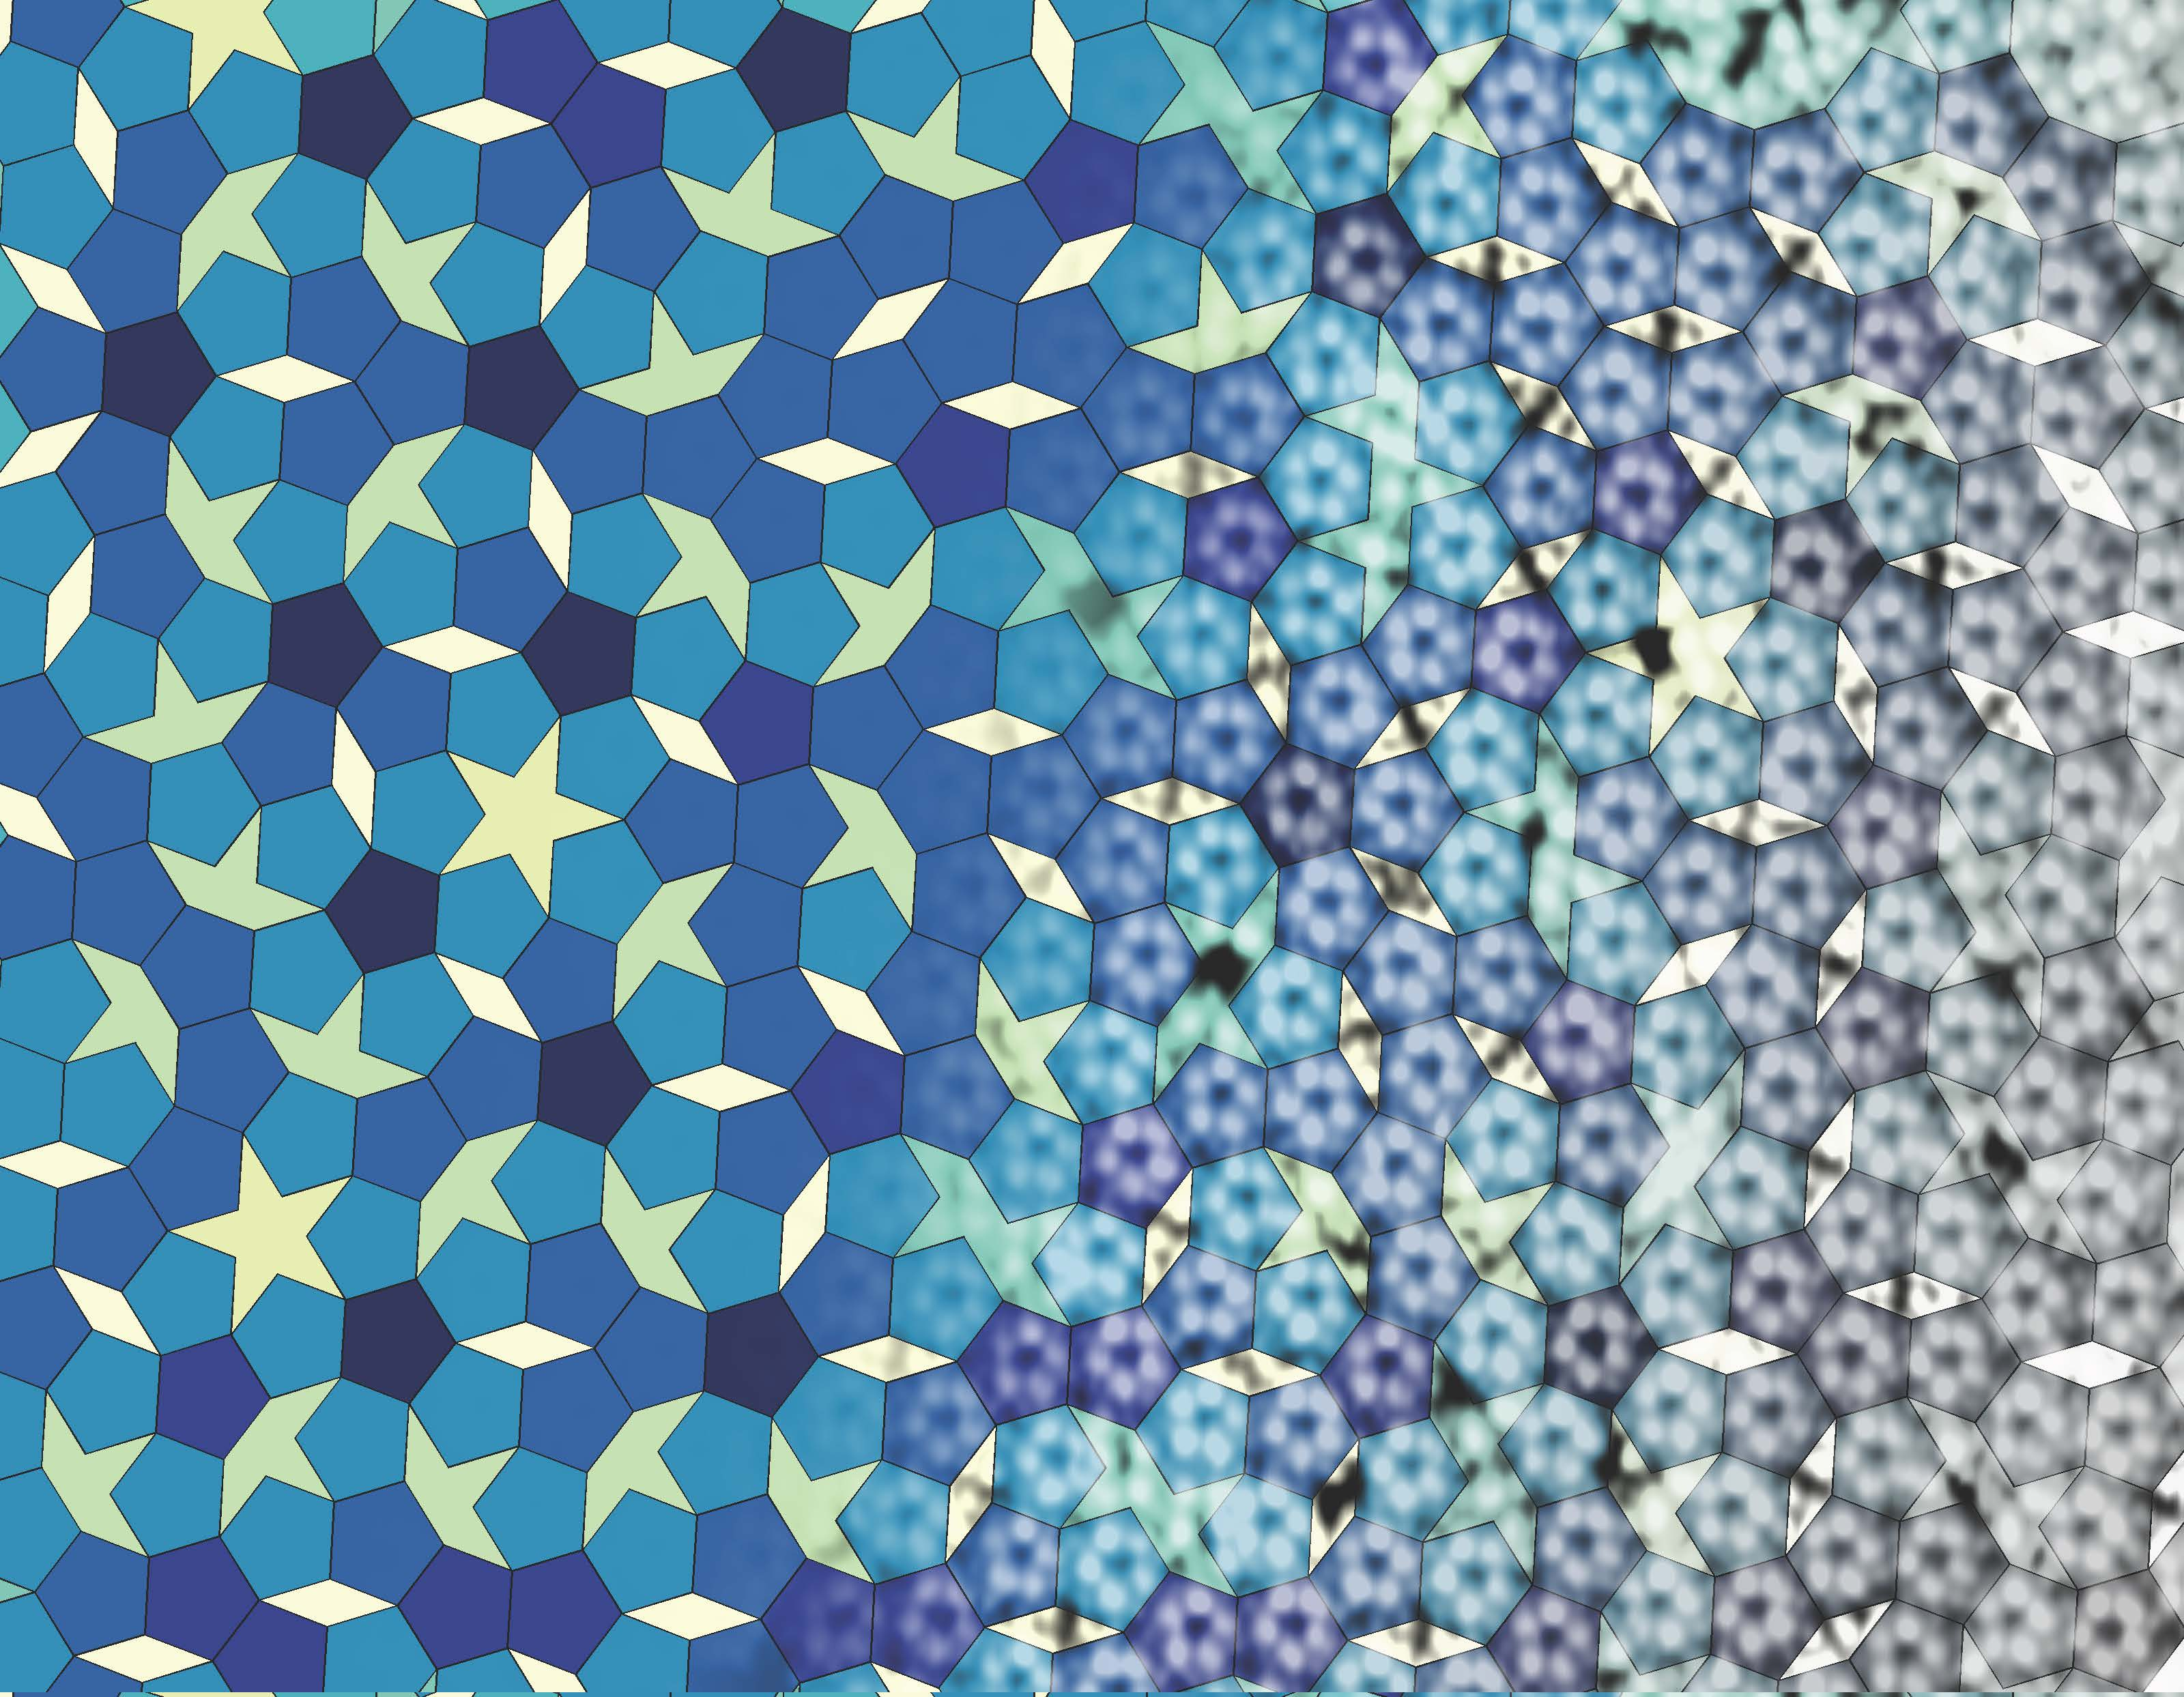
\includegraphics[scale=0.22]{img/wasio.jpg}
		
		\ss{A 2D hydrogen-bonded quasicrystal} \ss{(see \url{doi:10.1038/nature12993})}
	\>
\)

\begin{itemize}
	\item Numerous metallic and soft-matter quasicrystals have been synthetized
	\item only one natural example example is known: the Khatyrka meteorite (see \url{doi:10.1126/science.1170827 }). 
\end{itemize}
\end{frame}

\section{Diffraction}
\subsection{Dummy}
\begin{frame}{Diffraction by a qp lattice: a simple case}
\centering
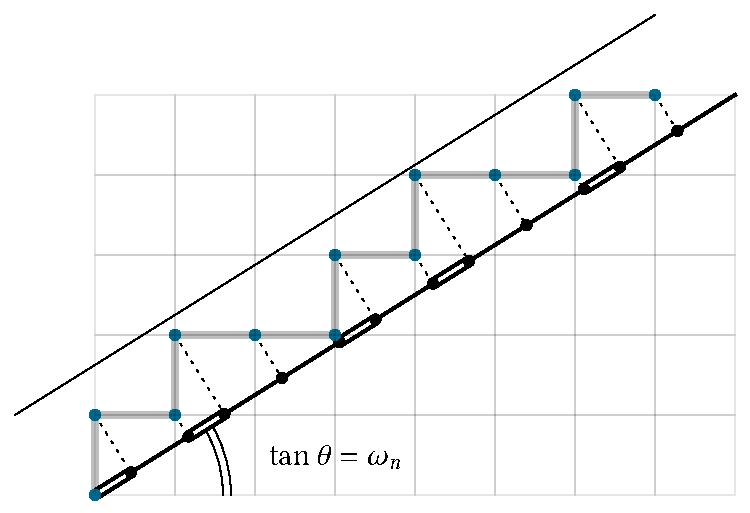
\includegraphics[scale=.8]{img/cut_and_project_diffraction.pdf}
\end{frame}

\begin{frame}{Diffraction by a qp lattice: a simple case}
\centering
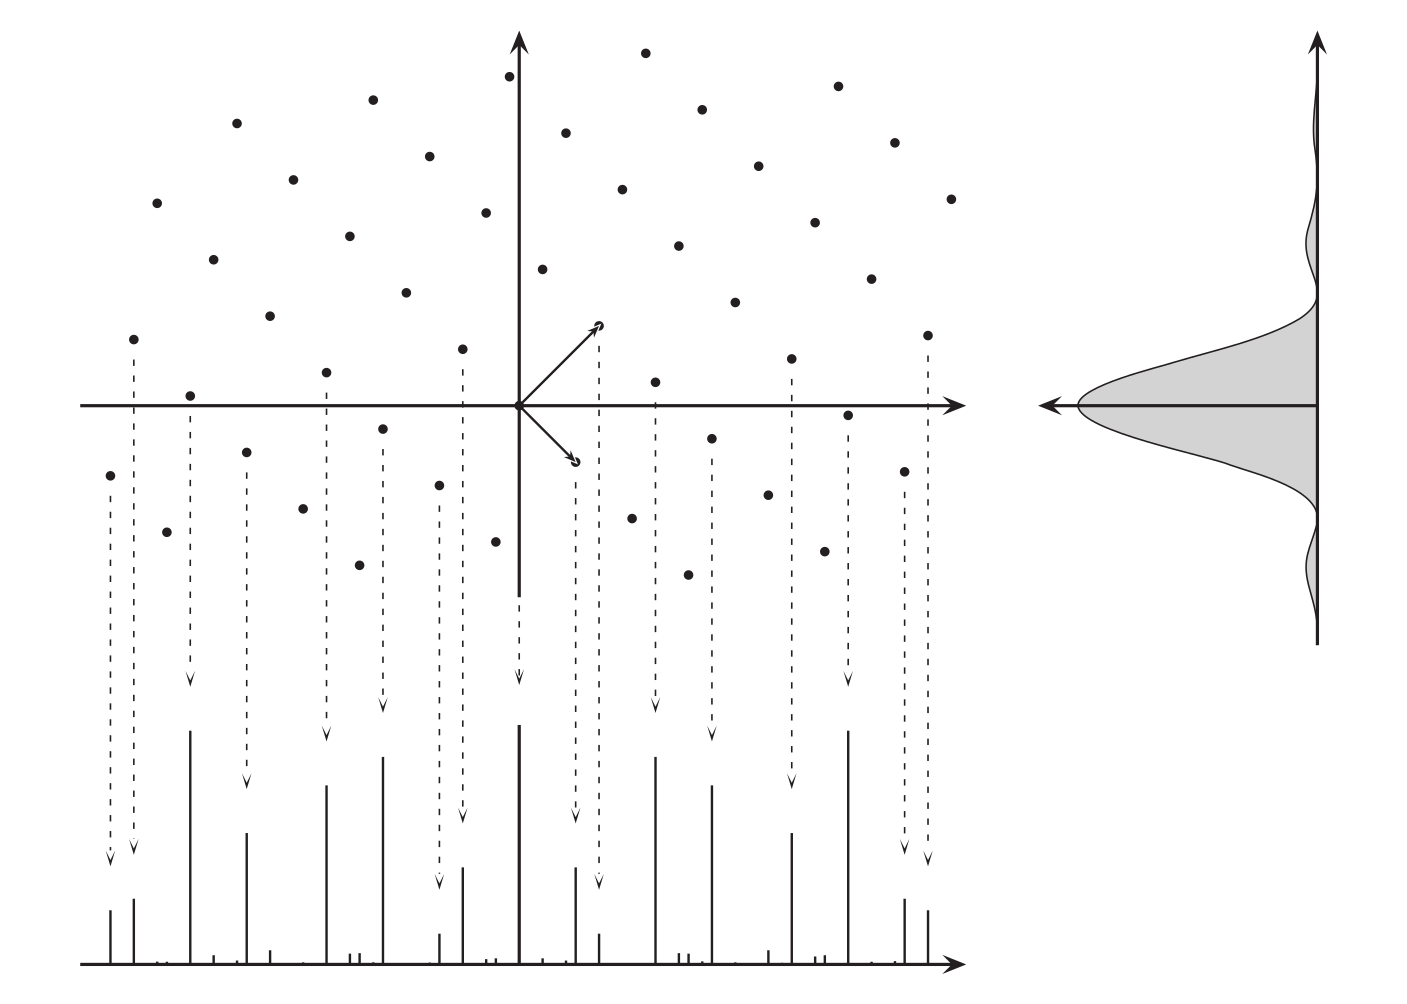
\includegraphics[scale=.2]{img/diffraction_silver_mean.png}
\end{frame}

\begin{frame}{Diffraction by a qp lattice}
\(
	\<{6cm}
		\centering
		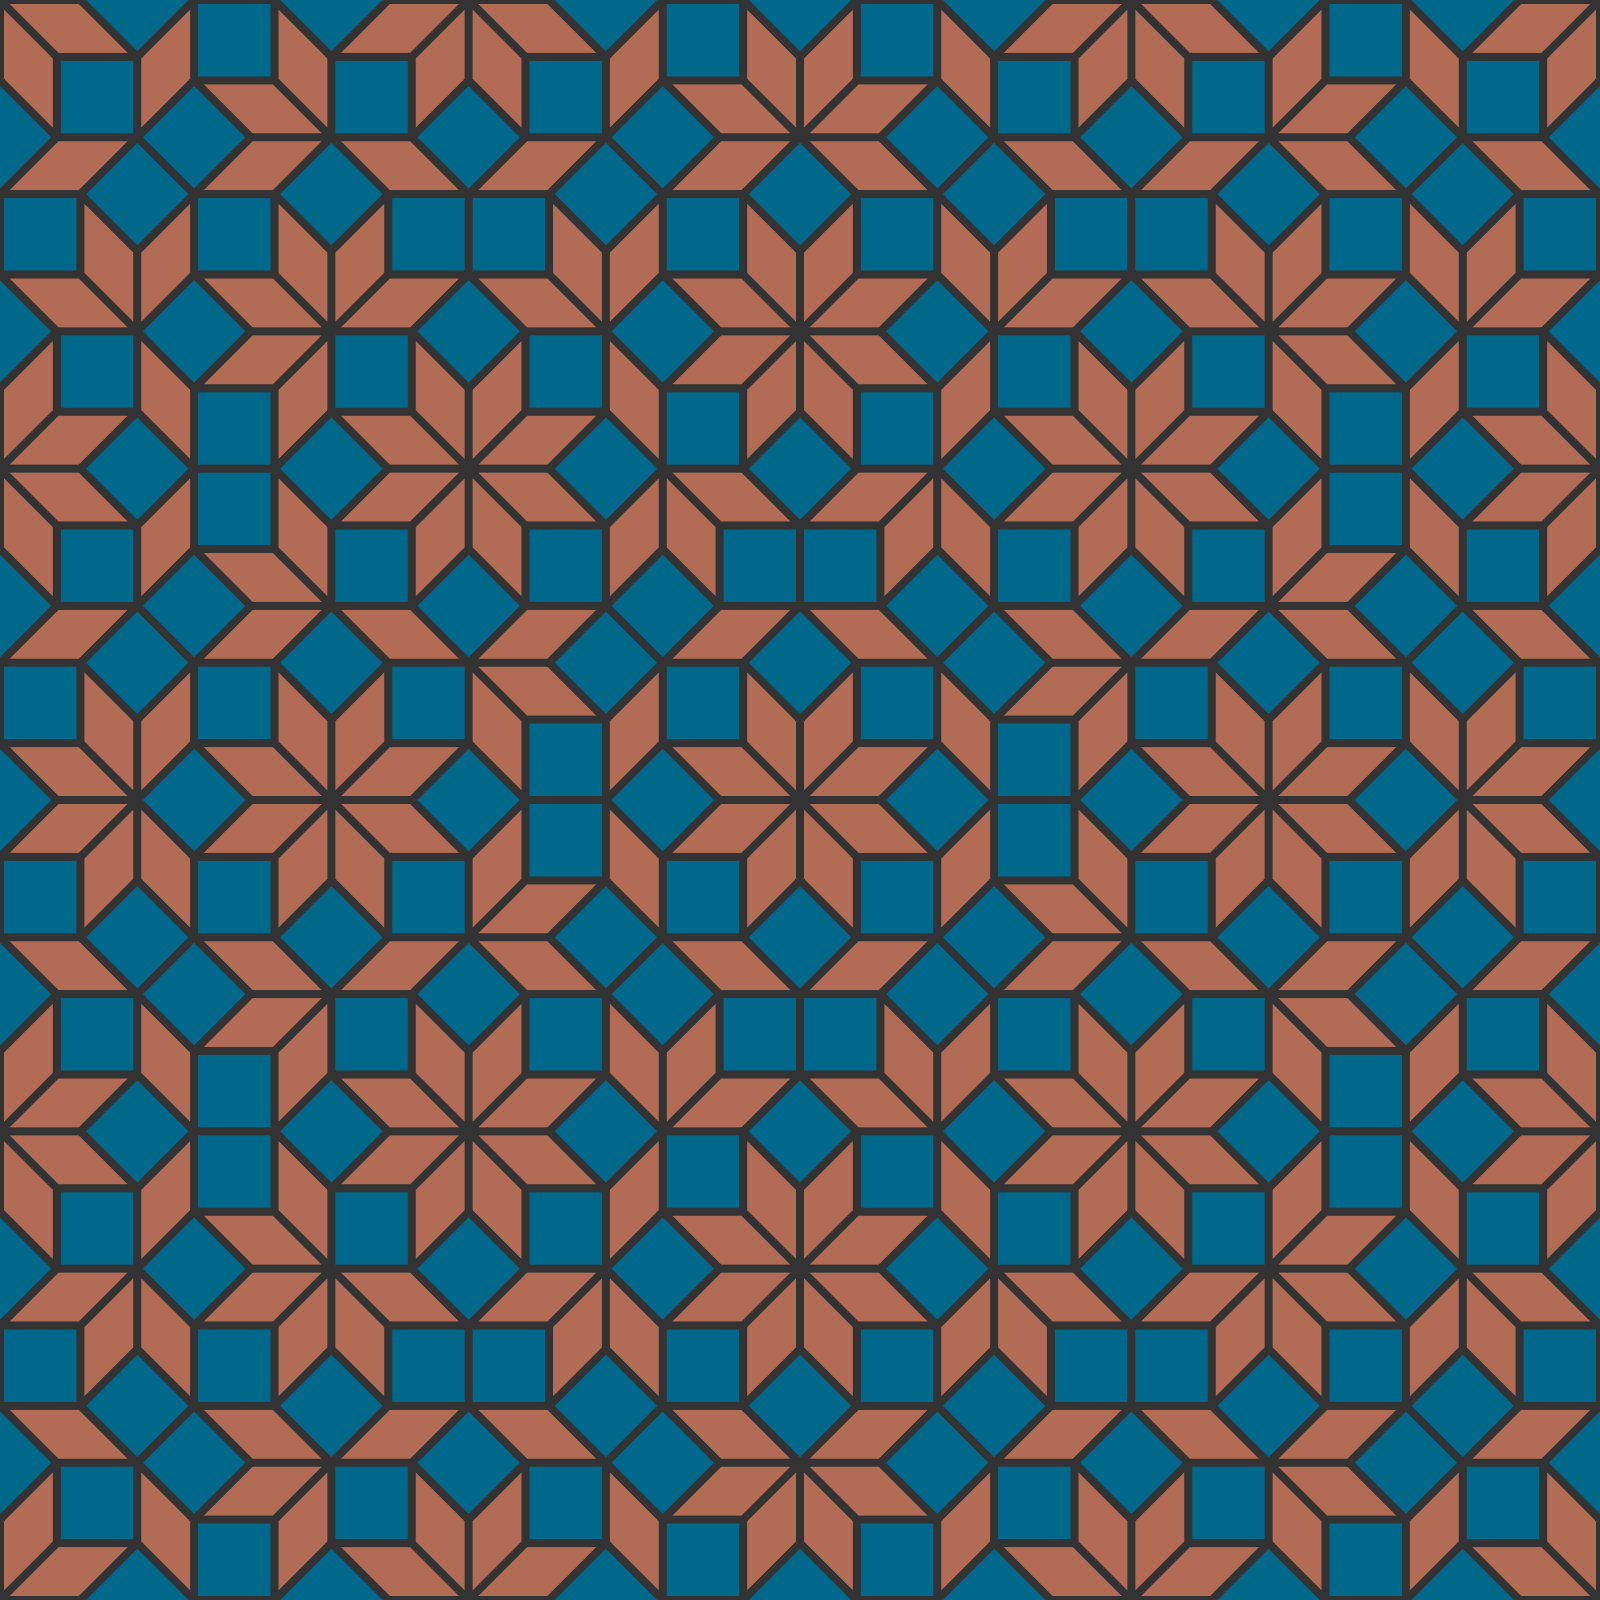
\includegraphics[scale=0.1]{img/ammann-beenker.png}
		
		\ss{The octagonal tiling...}
	\>
	\<{6cm}
		\centering
		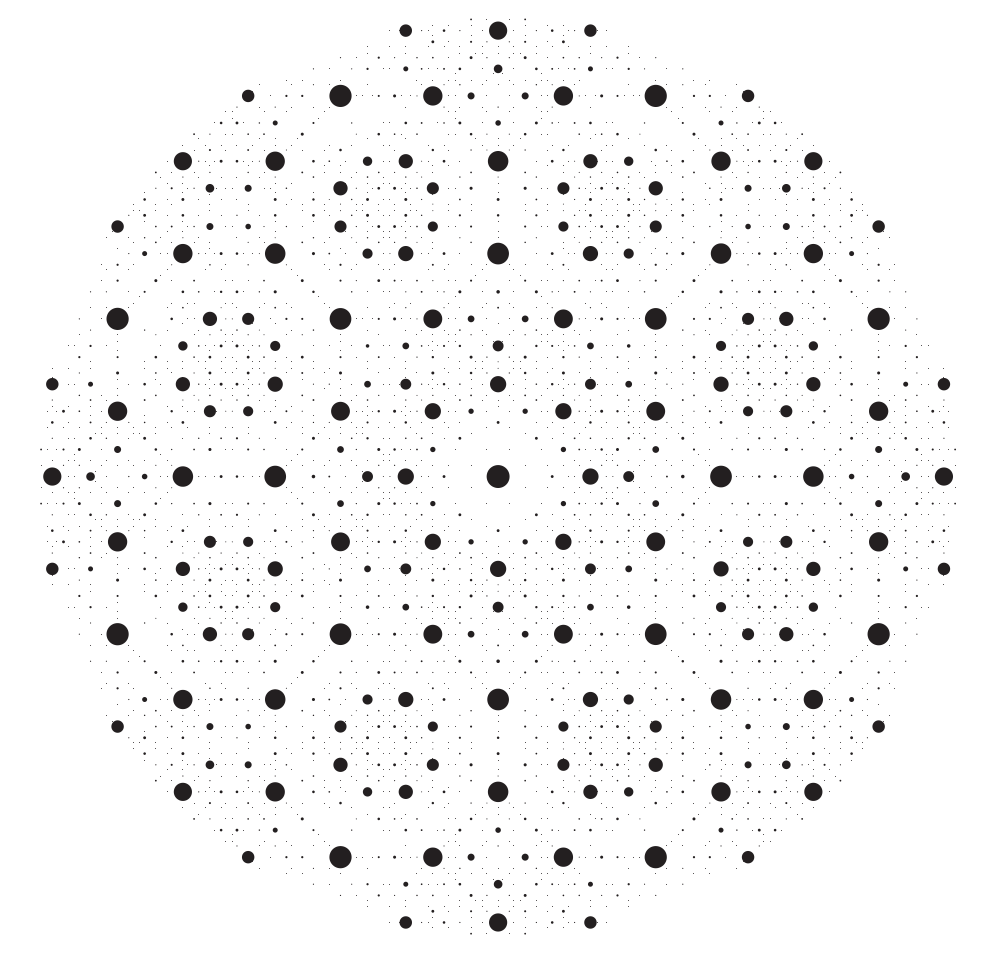
\includegraphics[scale=0.178]{img/diffraction_ammann_beenker.png}
		
		\ss{...and its diffraction pattern} \ss{(see \emph{Aperiodic Order}, Baake \& Grimm)}
	\>
\)
\end{frame}

\section{Electronic states on quasicrystals}
\subsection{Dummy}
\begin{frame}{A quasicrystal toy model: the Fibonacci chain}
\centering

\includegraphics[scale=1.2]{img/chain_for_inset.pdf}
\[
	H = \sum_i t_{i,i+1}(\ket{i}\bra{i+1} + \ket{i+1}\bra{i})
\]
\[
	t(=\joinrel=) = 1,~t(-) = \rho
\]

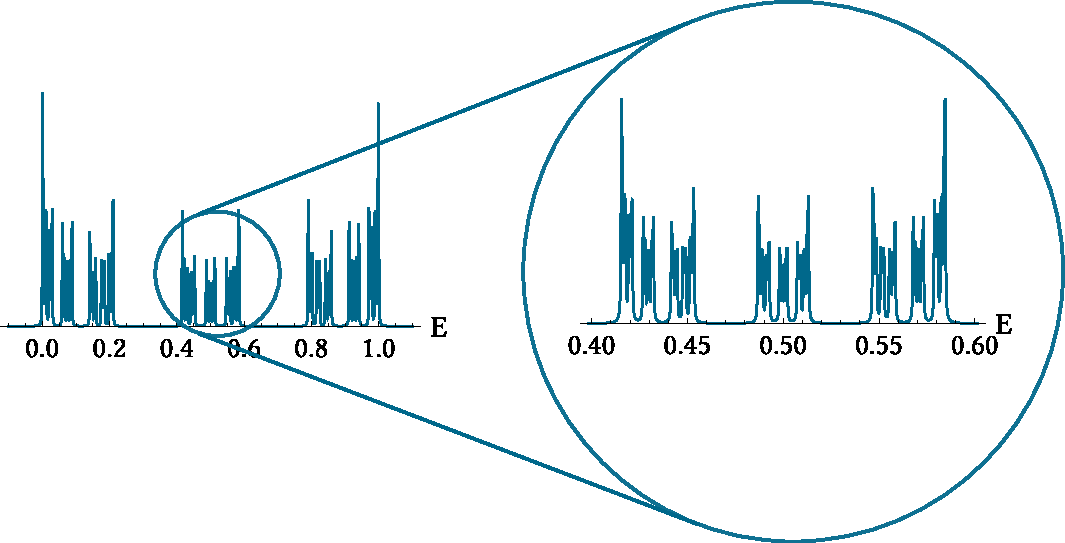
\includegraphics[scale=.5]{img/ldos.pdf}

The density of states of even  the simplest quasicrystal toy model is still complicated, and has an interesting fractal structure.
\end{frame}

\begin{frame}{The $E=0$ wavefunction}
\centering
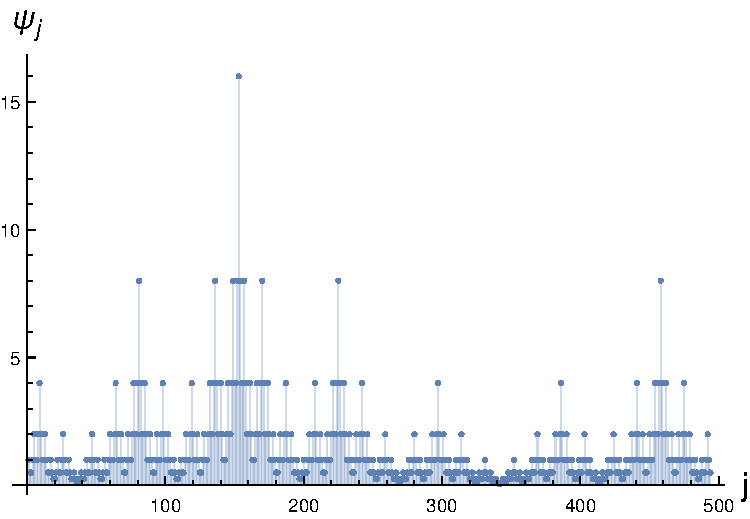
\includegraphics[scale=.8]{img/wavefunction.pdf}
\end{frame}

\begin{frame}{In 2D...}
\centering
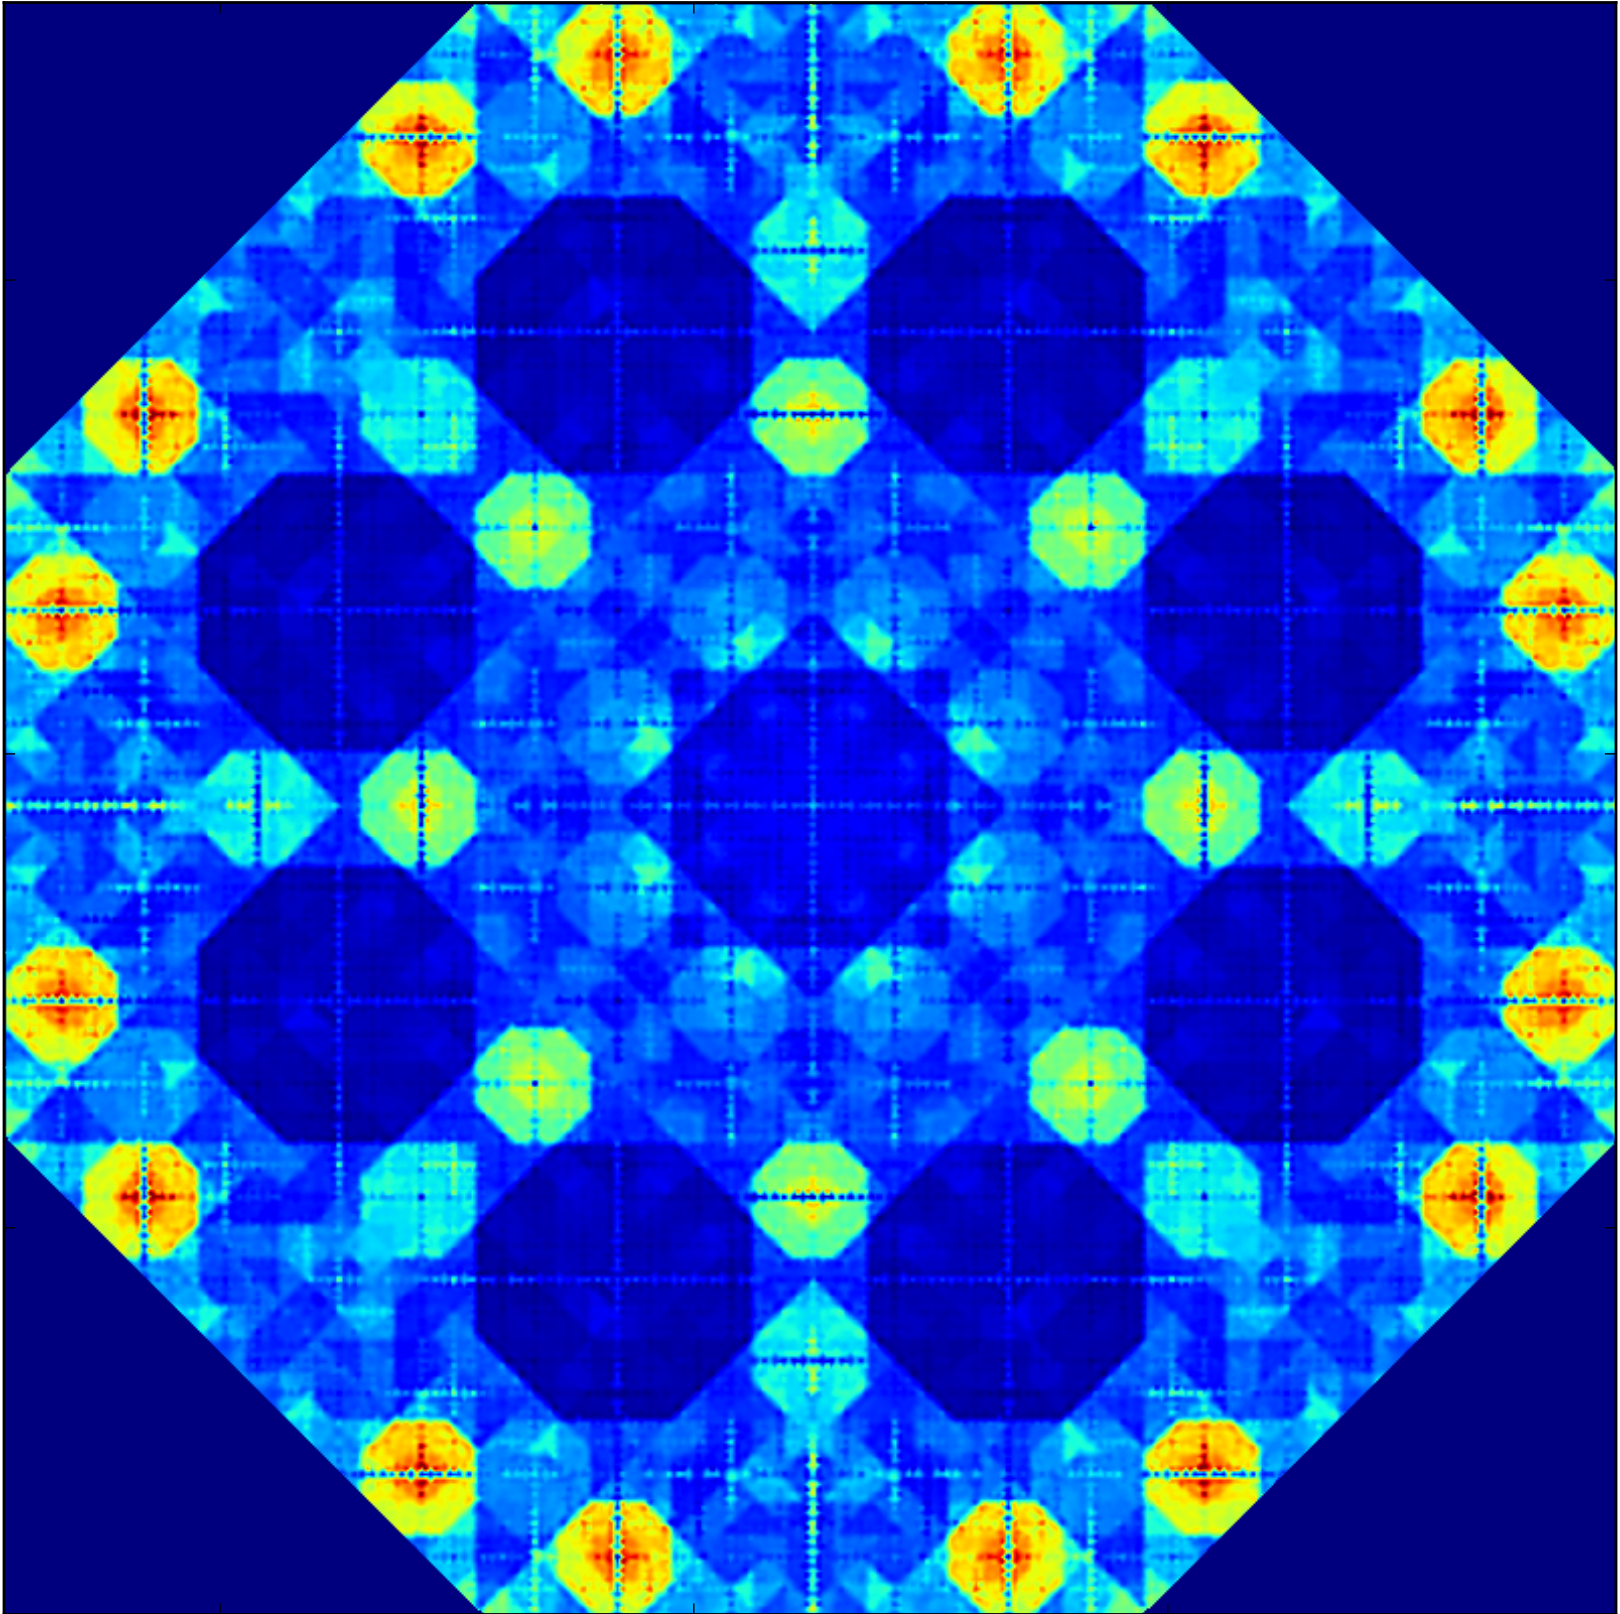
\includegraphics[scale=.35]{img/octagonal.png}

\ss{A state on the octagonal tiling}
\ss{(numerical simulation by Eric Adrade)}
\end{frame}

\section{Bonus: the gap labelling theorem}
\subsection{Dummy}
\begin{frame}{The electronic spectrum}
\centering
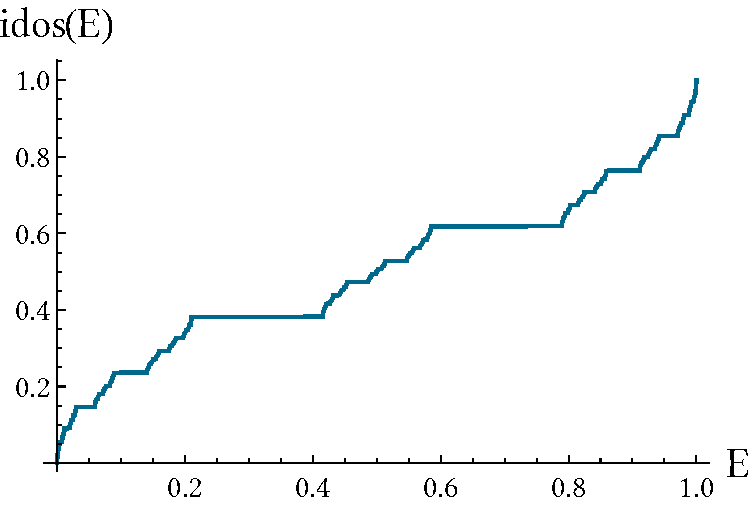
\includegraphics[scale=.7]{img/idos_fibonacci.pdf}

\ss{The integrated density of states (the fraction of states} \ss{below an energy $E$), for the Fibonacci chain.} 
\end{frame}

\begin{frame}{The electronic spectrum reinterpreted}
\centering
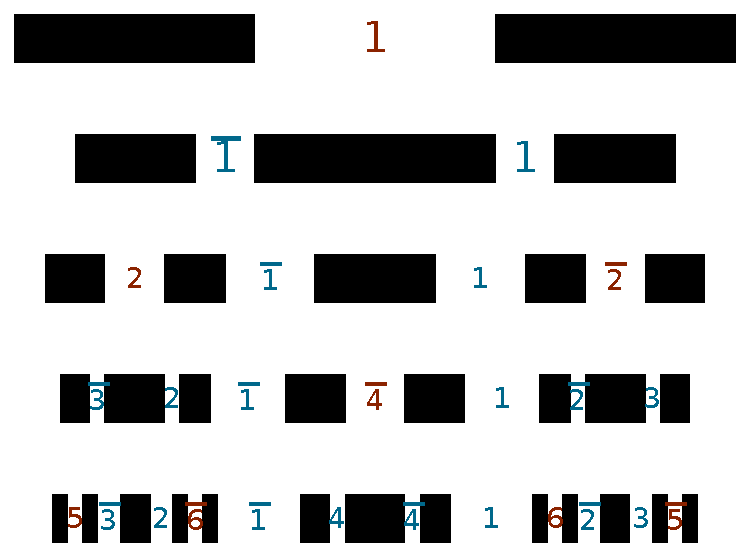
\includegraphics[scale=.7]{img/gap_labels.pdf}

\ss{The gap labels for increasingly large approximants to the Fibonacci chain.}
\end{frame}

\end{document}